\section{Scene Graph}
\label{chapter:implementation:scenegraph}

	The basic design of the base class for all specialized scene nodes is presented in Figure \ref{fig:SceneNode1}. Note that there are many more methods in the actual implementation that were only added for convenience. We will look at the implementation of all methods in this graph, dividing them into two categories:

	\begin{smalllist}
		\item Re-parenting
		\item Property Queries and Modifications
	\end{smalllist}

	We will additionally look into the implementation of some convenience methods and patterns that try to further simplify the API.

	\begin{figure}[htbp]
		\centering
		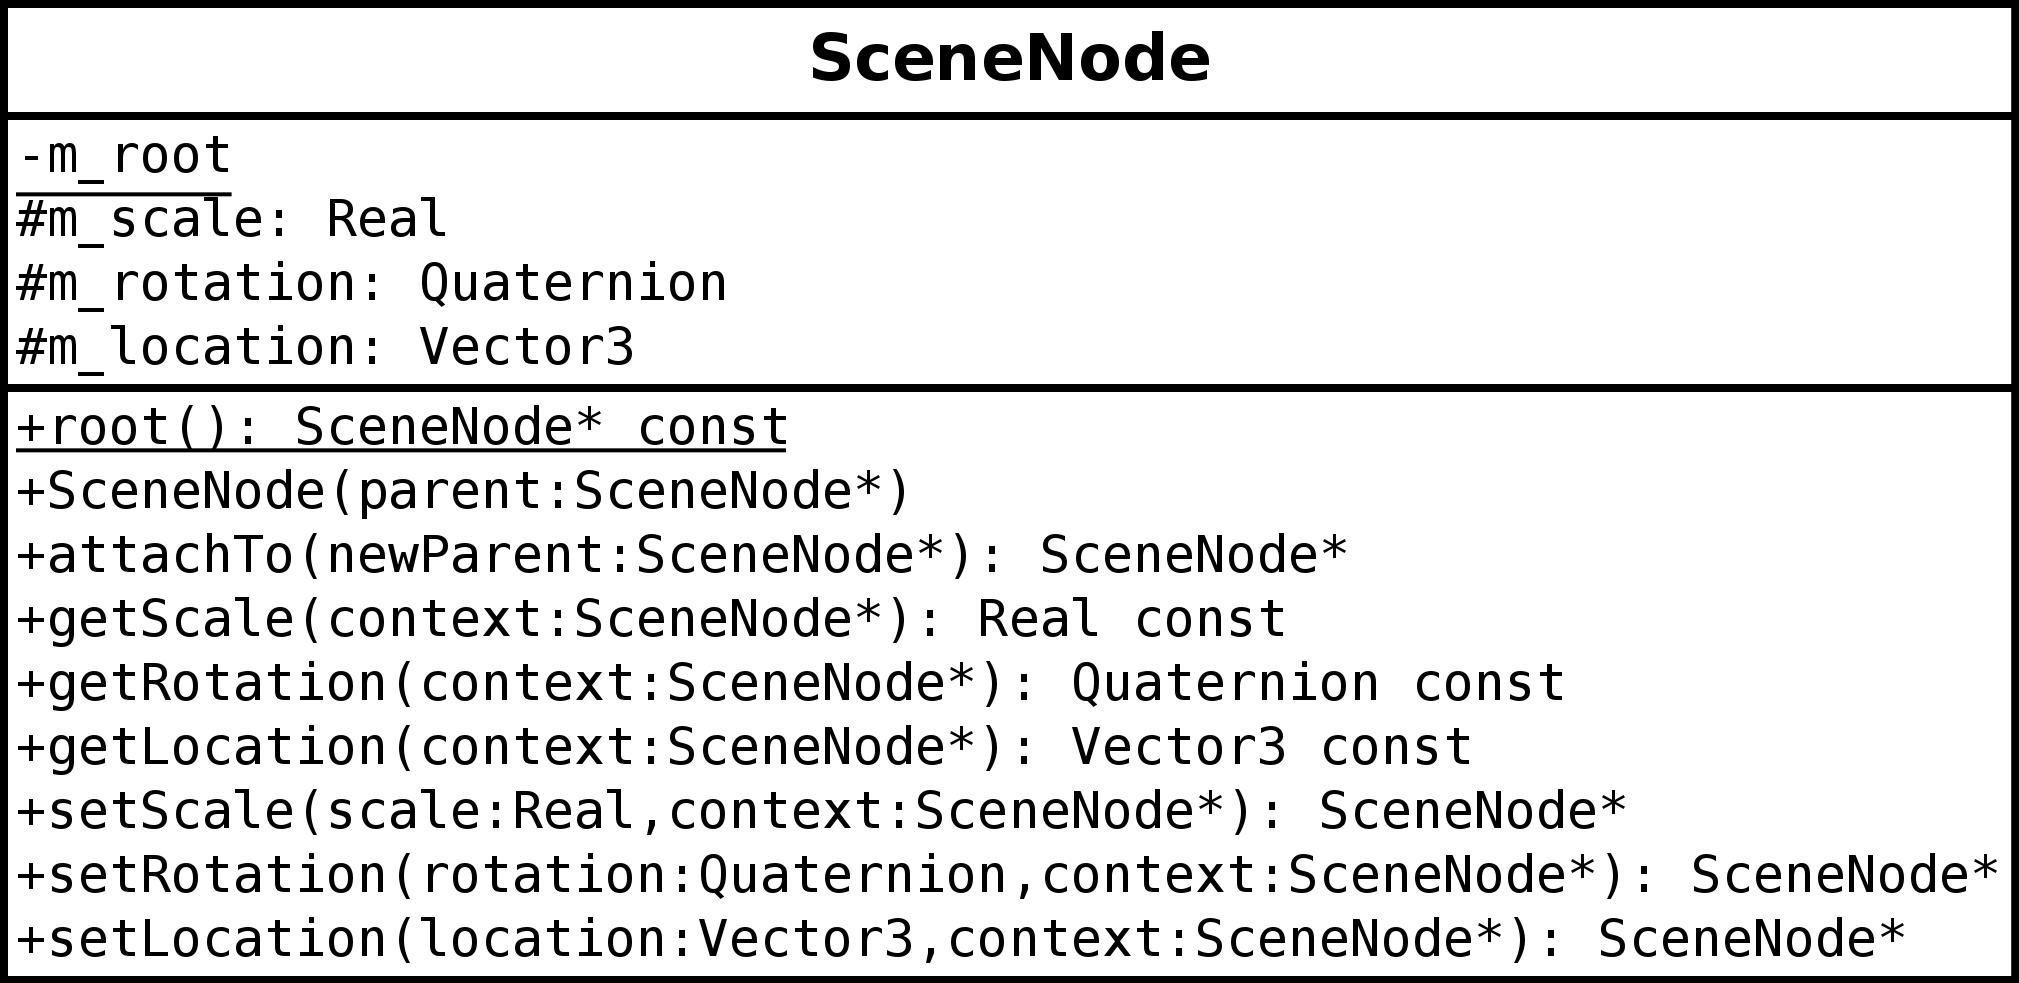
\includegraphics[width=10cm]{images/SceneNode1.png}
		\caption{Basic layout of the \classname{SceneNode} class.}
		\label{fig:SceneNode1}
	\end{figure}

	\subsection{Re-parenting}

		When arbitrary re-parenting of scene nodes is supported in an API, there is the possibility to create circular dependencies:

		\begin{code}[2]
			knifeNode->attachTo(forkNode);
			forkNode->attachTo(knifeNode);
		\end{code}

		We have three solutions to this issue: Either

		\begin{smalllist}
			\item the API is designed in a way that makes it impossible to create any circular dependencies,
			\item the issue is ignored altogether as such a circular construct is no longer part of the scene graph and does not have any impact on the visual output, or
			\item the library checks for them at certain points during the execution.
		\end{smalllist}

		The only available solution eliminating the problem altogether is the prohibition of re-parenting scene nodes. It is not possible to generate circular dependencies if an existing parent node is responsible for creating new nodes and those parents cannot be re-attached to other nodes. We will discard this very effective solution, as it renders the scene graph API very inflexible.

		The next option is to ignore such constructs. As every node has exactly one parent, a circle implies that it does not have a reference to the root scene node. Since the scene only contains nodes that are somehow attached to the root node, these nodes won't be displayed at all. This choice could lead to bugs that are quite hard to find for the same reason.

		The remaining option involves verifying the tree structure either when the scene graph changes or when the parent of a scene node is queried. Since the parent node is expected to change less often than it is queried, the check for circular references is performed immediately after an object is attached to another one. This choice additionally provides much more concise error messages and better supports debugging of such an error case.

	\subsection{Property Query and Modification}

		\subsubsection{Scale}

			The scale of a node in the global context is the product of all scale factors in all parent nodes: $s_g = s_{p_0} \cdot s_{p_1} \cdot \ldots \cdot s_{p_n} \cdot s_n$. Evaluating the scale of a scene node from the viewpoint of another node, we just need to find the quotient of the global scale values of the viewpoint and the queried node:

			\begin{code}[4]
				Real SceneNode::getScale(SceneNode* context) {
				    if (context == parent) {
				        return m_scale;
				    }
				    if (context == root()) {
				        return parent->getScale(root()) * m_scale;
				    }
				    return getScale(root()) / context->getScale(root());
				}
			\end{code}

			Although this implementation would be sufficient, we have added another dedicated if-block for handling the case where \inlinecode{context == this}, as the return value is always 1 in this case. Space never seems distorted from ones own viewpoint.
	
			After the implementation of the query method, the implementation of the setter becomes trivial:

			\begin{code}[4]
				SceneNode* SceneNode::setScale(Real s, SceneNode* context) {
				    m_scale *= s / getScale(context);
				    return this;
				}
			\end{code}

		\subsubsection{Rotation}

			Rotations are stored as a rotation within the coordinate system of the parent node. To evaluate the rotation of a scene node in the global context, we will need to multiply the rotations of all parent nodes. The return value of \inlinecode{node->getRotation(RootSceneNode::get())} is computed by $r_g = r_{p_0} \cdot r_{p_1} \cdot \ldots \cdot r_{p_n} \cdot r_n$, where $r_n$ denotes the rotation quaternion of the current node and $r_{p_0}$ through $r_{p_n}$ are the rotation quaternions of the parent nodes.

			To evaluate the rotation of a node in the coordinate system of another node, we can take the rotations of both nodes in the global coordinate system and compute the necessary quaternion that would change the rotation of the viewpoint to that of the target. If $r_g$ and $R_g$ are the global rotation quaternions of the target and context nodes respectively, the rotation from $R_g$ to $r_g$ can be computed using $\Delta r = R_g^{-1} \cdot r_g$.

			The resulting quaternion $\Delta r$ can be used to rotate $R_g$ to $r_g$, as $R_g \cdot \Delta r = R_g \cdot R_g^{-1} \cdot r_g = r_g$. Surprisingly the steps required for this computation do not differ from the evaluation of the scale. This defines the implementation of \inlinecode{getRotation()} method very similar to \inlinecode{getScale()}:

			\begin{code}[4]
				Quaternion SceneNode::getRotation(SceneNode* context) {
				    if (context == parent) {
				        return m_rotation;
				    }
				    if (context == root()) {
				        return parent->getRotation(root()) * m_rotation;
				    }
				    return context->getRotation(root()).inverse() *
			            getRotation(root());
				}
			\end{code}

			The method for updating the rotation is analogous to \inlinecode{setScale} as well:

			\begin{code}[4]
				SceneNode* SceneNode::setRotation(Quaternion r, SceneNode* context) {
				    Quaternion perceivedRot = getRotation(context);
				    m_rotation *= perceivedRot.inverse() * r * perceivedRot;
				    return this;
				}
			\end{code}

		\subsubsection{Location}

		Finding the location of an object is a bit more complex, as the calculation involves the other two properties. The position in global space is defined by \[l_g = l_{p_0} + (r_{p_0} \cdot l_{p_1} \cdot s_{p_0}) + \ldots + (r_{p_{n-1}} \cdot l_{p_n} \cdot s_{p_{n-1}}) + l_n\] This is necessary as the \emph{rotation} and \emph{scale} properties do not effect the node they have been defined in but solely effect the sub-space they are creating.

			This makes the calculation of a relative location to another more complex as well. After finding the global positions of both nodes (the queried node and the context node), we can create a vector pointing from one point to the other. We will need to adjust that vector using the rotation and scale of the own values of the context node: \[\Delta l = R_n \cdot (l_g - L_g) \cdot S_n\]

			After that we can use $\Delta l$ to position an object in the space of the context node at the exact same position as the initially queried node. The implementation of this method explicitly requires the handling of the context node being the parent node this time:

			\begin{code}[4]
				Vector3 SceneNode::getLocation(SceneNode* context) {
				    if (context == parent) {
				        return m_location;
				    }
				    if (context == root()) {
				        return parent->getLocation(root()) +
				               parent->m_rotation * m_location * parent->m_scale;
				    }
				    return getLocation(root()) - context->getLocation(root());
				}
			\end{code}

			Setting the location from an external viewpoint is as simple as the setter of the other two properties:
			
			\begin{code}[4]
				SceneNode* SceneNode::setLocation(Vector3 l, SceneNode* context) {
					m_location += l - getLocation(context);
				    return this;
				}
			\end{code}

	\subsection{Convenience}

		\subsubsection{Additional Methods}

			The methods presented at the beginning of this Section are completely sufficient to perform all available operations on \classname{SceneNode}s. Being limited to these few operations would render the API unnecessarily complex. We will try to hide any design details until the developer actively seeks them out. We have implemented a wide variety of additional methods for this purpose:

			\begin{smalllist}
				\item Property modification without context, where the context is assumed to be the parent node:
				\begin{smalllist}
					\item setScale(Real scale)
					\item setRotation(Quaternion rotation)
					\item setLocation(Vector3 location)
				\end{smalllist}
				\item Relative property modification:
				\begin{smalllist}
					\item scale(Real scalar)
					\item rotate(Quaternion rotation)
					\item move(Vector3 vector)
				\end{smalllist}
				\item Relative movement and rotation, both with and without the additional context parameter:
					\begin{smalllist}
						\item \begin{tabular}{|l}
								moveLeft(Real amount) \\ moveRight(Real amount)
							\end{tabular}
						\item \begin{tabular}{|l}
								moveUp(Real amount) \\ moveDown(Real amount)
							\end{tabular}
						\item \begin{tabular}{|l}
								moveForward(Real amount) \\ moveBackward(Real amount)
							\end{tabular}
						\item \begin{tabular}{|l}
								rotateLeft(Angle amount) \\ rotateRight(Angle amount) \\ turnLeft(Angle amount) \\ turnRight(Angle amount)
							\end{tabular}
						\item \begin{tabular}{|l}
								rotateUp(Angle amount) \\ rotateDown(Angle amount) \\ turnUp(Angle amount) \\ turnDown(Angle amount)
							\end{tabular}
						\item \begin{tabular}{|l}
								tiltLeft(Angle amount) \\ tiltRight(Angle amount)
							\end{tabular}
					\end{smalllist}
			\end{smalllist}

			The definition of these methods have bloated the API on one hand, but provided the perfect method for many use cases. We have noticed during testing that we were not using quaternions at all. We were able to create our test scenes just with relative modification of our objects.

		\subsubsection{Fluent Interfaces}

			When embedding an object into the scene graph, we need to adjust several properties of the object. Usually this involves multiple distinct calls to a newly created scene node. A pattern that we immediately thought of with this insight was the fluent interface\cite{Fowler2010}. Fluent interfaces return the object that is being operated on to allow us to chain multiple methods. The above example would be reduced to just four lines of code with the implementation of this idea:

			% whitespace
			\begin{code}[4]
				table = Model::create("Table");
				cutlery = SceneNode::create()
				    ->setPosition(1, 1, 10)
				    ->attachTo(table);
				knife = Model::create("Knife")
				    ->setPosition(1, 0, 0);
				    ->attachTo(cutlery);
				fork = Model::create("Fork")
				    ->attachTo(cutlery);
			\end{code}

			Unfortunately, we had chosen to sub-class the \classname{SceneNode} for each object type that can be attached to the scene graph. This means that any operation on the \classname{SceneNode} API would return a \classname{SceneNode} object and no longer its sub-class. But a fluent API returning the covariant type would be much more intuitive to avoid the following scenario:
			
			% whitespace
			\begin{code}[4]
				light = SpotLight::create()
				    // the next call would return a SceneNode object
				    // which does not provide the setColor() method:
				    ->setPosition(1, 1, 1)
				    // compilation error on the next line:
				    ->setColor(Color::RED);
			\end{code}

			The simplest solution would be to re-implement all methods of the \classname{SceneNode} in the \classname{SpotLightNode} class to return the type of the implementing class. Instead of performing this implementation in each sub-class of \classname{SceneNode}, we will use the \emph{curiously recurring template pattern} (CRTP) to accomplish this task. \cite{Lippman:1996:CG:260627} presents this pattern based on work in \cite{Barton:1994:SEC:561392} and its implementation in our library is presented in Figure \ref{fig:FluentInterface}

			\begin{figure}[htbp]
				\centering
				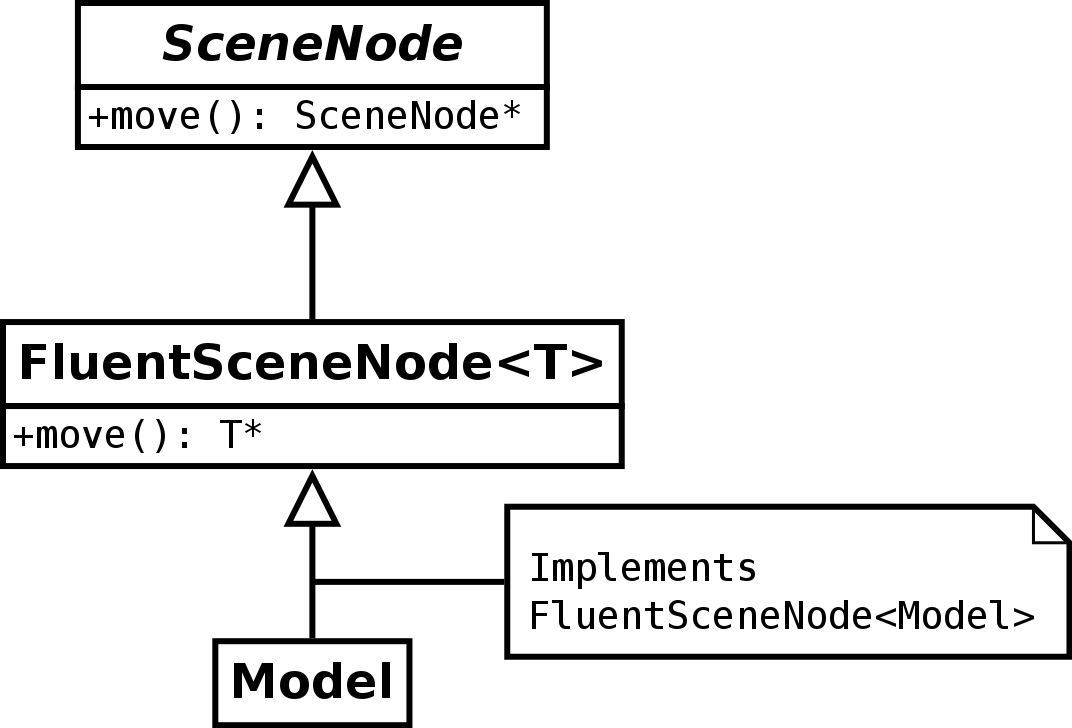
\includegraphics[width=8cm]{images/FluentInterface.png}
				\caption{The architecture of the fluent interface. The template class' method \inlinecode{FluentSceneNode<T>::move()} executes \inlinecode{SceneNode::move()} and returns \inlinecode{this}, casting it to a \inlinecode{T} pointer.}
				\label{fig:FluentInterface}
			\end{figure}

			The API now returns the type of the object an operation was called on, allowing us to use all methods of a \classname{SpotLightNode} in succession, regardless of the implementation of the methods within the class hierarchy.

